% vim: set ft=tex tabstop=4 shiftwidth=4 noexpandtab:

% header %{{{1

% opening %{{{2

\documentclass[tikz, border=1mm]{standalone}

% packages and libraries %{{{2

% ---- not necessary since the documentclass[tikz ...] requires it automatically
% \usepackage{tikz}

\usepackage{amsmath}
\usepackage{mathrsfs}
\usepackage[x11names]{xcolor}

\usetikzlibrary{calc,angles,quotes,intersections,shapes.geometric}

\usepackage{tkz-euclide}

% colors %{{{2

\definecolor{goldenbrown}{HTML}{5b3c11}

%\definecolor{somebrown}{RGB}{101,67,33}

%\colorlet{somebrown}{brown!80!black}

% style %{{{2

\tikzset{
	% ---- default
	every path/.style={line width=0.3pt},
	every coordinate/.style={fill=black, circle, inner sep=1pt},
	every node/.style={font=\normalsize},
	every picture/.style={scale=1.0},
	% ---- custom
	construction/.style={line width=0.1pt, dashed},
	dimension/.style={line width=0.2pt, <->, goldenbrown},
	dimension extension/.style={line width=0.2pt, dashed, goldenbrown},
	vector/.style={->, thick},
}

% document %{{{1

% opening %{{{2

\begin{document}
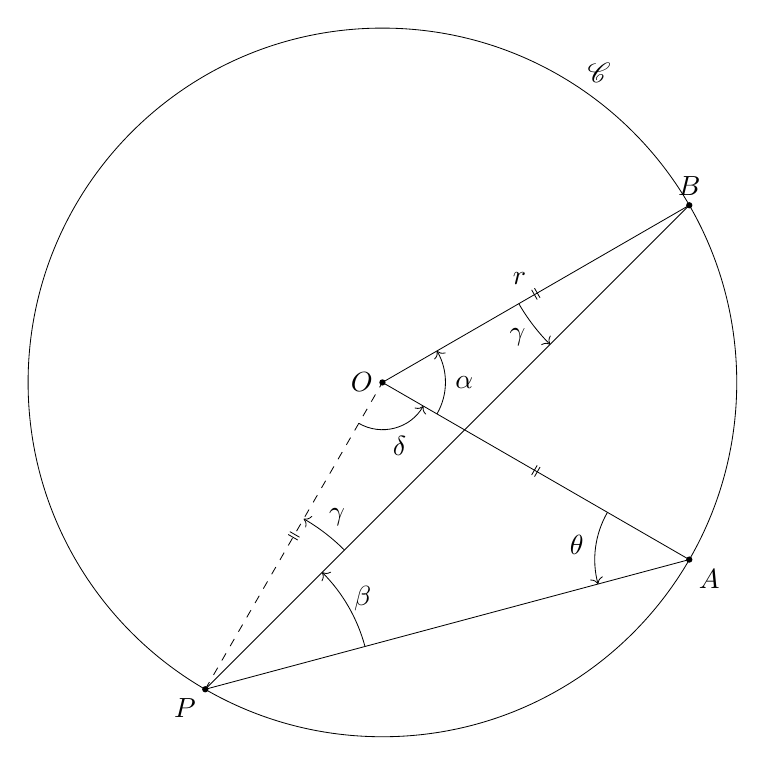
\begin{tikzpicture}[scale=1.0]

% parameters %{{{2

	\def\ang{-30}
	\def\gle{30}
	\def\ngl{240}

	\def\radius{4.5}

% coordinates %{{{2

	\coordinate (O) at (0,0);
	\coordinate (A) at (\ang:\radius);
	\coordinate (B) at (\gle:\radius);
	\coordinate (P) at (\ngl:\radius);

% points, dots, vertices %{{{2

	\fill (O) circle (0.4mm);
	\fill (A) circle (0.4mm);
	\fill (B) circle (0.4mm);
	\fill (P) circle (0.4mm);

% segments, sides %{{{2

	\draw (O) -- (A);
	\draw (O) -- (B);
	\draw[dashed] (P) -- (O);
	\draw (P) -- (A);
	\draw (P) -- (B);

% circles %{{{2

	\draw (O) circle (\radius);

% points, dots, vertices labels %{{{2

	\node[left] at (O) {$O$};
	\node[below right] at (A) {$A$};
	\node[above] at (B) {$B$};
	\node[below left] at (P) {$P$};

% segments, sides labels %{{{2

	\node[above left] at ($ (O)!0.5!(B) $) {$r$};

% segments, sides marks %{{{2

	\tkzMarkSegments[mark=||, size=2pt](O,A)
	\tkzMarkSegments[mark=||, size=2pt](O,B)
	\tkzMarkSegments[mark=||, size=2pt](O,P)

% circle label %{{{2

	\node at (55:{\radius+0.3}) {$\mathscr{C}$};

% angles labels %{{{2

	\pic[draw, ->, "$\alpha$", angle radius=0.8cm, angle eccentricity=1.3]
	{angle = A--O--B};

	\pic[draw, ->, "$\beta$", angle radius=2.1cm, angle eccentricity=1.1]
	{angle = A--P--B};

	\pic[draw, ->, "$\gamma$", angle radius=2.5cm, angle eccentricity=1.1]
	{angle = B--P--O};

	\pic[draw, ->, "$\gamma$", angle radius=2.5cm, angle eccentricity=1.1]
	{angle = O--B--P};

	\pic[draw, ->, "$\theta$", angle radius=1.2cm, angle eccentricity=1.2]
	{angle = O--A--P};

	\pic[draw, ->, "$\delta$", angle radius=0.6cm, angle eccentricity=1.4]
	{angle = P--O--A};

% closing %{{{2

\end{tikzpicture}
\end{document}
